\documentclass[11pt]{article}
\usepackage[utf8]{inputenc}
\usepackage[margin=2cm]{geometry}
\usepackage{longtable}
\usepackage{array}
\usepackage{booktabs}
\usepackage{multirow}
\usepackage{graphicx}
\graphicspath{{figures/}}
\usepackage{xcolor}
\usepackage{pdflscape}
\usepackage{caption}
\usepackage{enumitem}
\usepackage{fancyhdr}
\usepackage{titlesec}
\usepackage{tcolorbox}
\usepackage{colortbl}
\usepackage{microtype}
\usepackage{fontspec}
\usepackage{setspace}

\setmainfont{Times New Roman}
\setsansfont{Arial}

\definecolor{natureteal}{RGB}{0, 133, 124}
\definecolor{naturelightgray}{RGB}{245, 245, 245}
\definecolor{naturegray}{RGB}{100, 100, 100}

\titleformat{\section}
  {\normalfont\Large\bfseries\color{natureteal}}
  {\thesection}{1em}{}

\pagestyle{fancy}
\fancyhf{}
\fancyhead[L]{mLLMCelltype}
\fancyhead[R]{Supplementary Information}
\fancyfoot[C]{\thepage}
\renewcommand{\headrulewidth}{0.4pt}
\renewcommand{\footrulewidth}{0.4pt}
\setlength{\headheight}{14pt}
\captionsetup{font=small,labelfont=bf,textfont=it,labelsep=period}

\begin{document}

\begin{center}
\textcolor{natureteal}{\LARGE\textbf{Supplementary Information}}
\end{center}
\vspace{0.5cm}
\begin{center}
\textit{Large Language Model Consensus Substantially Improves the Cell Type Annotation Accuracy for scRNA-seq Data}
\end{center}
\vspace{0.3cm}
\begin{center}
Chen Yang\textsuperscript{1}, Xianyang Zhang\textsuperscript{1,*}, Jun Chen\textsuperscript{2,*}
\end{center}
\vspace{0.2cm}
\begin{center}
\small
\textsuperscript{1}Department of Statistics, Texas A\&M University, College Station, Texas 77843, USA\\
\textsuperscript{2}Division of Computational Biology, Department of Quantitative Health Sciences, Mayo Clinic, Rochester, Minnesota 55905, USA\\
\textsuperscript{*}Corresponding authors: zhangxiany@stat.tamu.edu, Chen.Jun2@mayo.edu
\end{center}
\vspace{1cm}

\section*{Supplementary Tables}

% Supplementary Table 1
\begin{landscape}
\begin{spacing}{1.1}
\begin{longtable}{>{\raggedright\arraybackslash}p{2.5cm}>{\raggedright\arraybackslash}p{3cm}>{\raggedright\arraybackslash}p{15cm}}
\caption*{\textbf{Supplementary Table 1 | Complete collection of prompt templates used in our multi-LLM consensus framework}, organized by function with full prompt text and explanations of key components.} \\
\toprule
\rowcolor{naturelightgray}
\textbf{Stage} & \textbf{Purpose} & \textbf{Template} \\
\midrule
\endfirsthead

\multicolumn{3}{c}{{\tablename\ \thetable{} -- continued from previous page}} \\
\toprule
\rowcolor{naturelightgray}
\textbf{Stage} & \textbf{Purpose} & \textbf{Template} \\
\midrule
\endhead

\midrule
\multicolumn{3}{r}{{Continued on next page}} \\
\endfoot

\bottomrule
\endlastfoot

\textbf{Initial Annotation} & Generate initial cell type predictions based on marker genes &
\begin{tcolorbox}[colback=white,colframe=naturelightgray,boxrule=0.5pt,arc=0pt,left=5pt,right=5pt,top=5pt,bottom=5pt]
\footnotesize
You are a cell type annotation expert. Below are marker genes for different cell clusters in [tissue\_name].

1: [gene\_list\_1]
2: [gene\_list\_2]
...

For each numbered cluster, provide only the cell type name in a new line, without any explanation.
\end{tcolorbox} \\
\midrule

\textbf{Consensus Checking} & Analyze predictions and calculate uncertainty metrics &
\begin{tcolorbox}[colback=white,colframe=naturelightgray,boxrule=0.5pt,arc=0pt,left=5pt,right=5pt,top=5pt,bottom=5pt]
\footnotesize
You are a cell type annotation expert. Below are different models' predictions for the same cell cluster.
Your task is to analyze these predictions and calculate uncertainty metrics.

\textbf{PREDICTIONS:}
Model 1: [prediction\_1]
Model 2: [prediction\_2]
...

\textbf{IMPORTANT GUIDELINES:}
1. Consider predictions as matching if they refer to the same cell type, ignoring differences in:
   - Formatting (e.g., 'NK cells' vs 'Natural Killer cells')
   - Capitalization
   - Additional qualifiers (e.g., 'activated', 'mature', etc.)
2. Group predictions that refer to the same cell type
3. If any prediction is 'Unknown' or 'Unclear', treat it as a separate group

\textbf{CALCULATE THE FOLLOWING METRICS:}
1. Consensus Proportion = Number of models supporting the majority prediction / Total number of models
2. Shannon Entropy = -sum(p\_i * log2(p\_i)) where p\_i is the proportion of models predicting each unique cell type
3. Determine if consensus is reached (Consensus Proportion > 2/3 AND Entropy <= 1.0)

\textbf{RESPONSE FORMAT:}
Line 1: 1 if consensus is reached, 0 if not
Line 2: Consensus Proportion (a decimal between 0 and 1)
Line 3: Shannon Entropy (a decimal number)
Line 4: The majority cell type prediction
\end{tcolorbox} \\
\midrule

\textbf{First Round Discussion} & Initial reasoning for cell type prediction using Toulmin model &
\begin{tcolorbox}[colback=white,colframe=naturelightgray,boxrule=0.5pt,arc=0pt,left=5pt,right=5pt,top=5pt,bottom=5pt]
\footnotesize
We are analyzing cluster [cluster\_id] with the following marker genes: [cluster\_genes] from [tissue\_name]
Different models have made different predictions:
[model\_1]: [prediction\_1]
[model\_2]: [prediction\_2]
...

Please provide your cell type prediction using the Toulmin argumentation model to structure your response:

1. \textbf{CLAIM:} State your clear cell type prediction (e.g., 'This is a T cell')
2. \textbf{GROUNDS/DATA:} Present specific observable evidence that supports your claim (e.g., marker genes expressed in this cluster)
3. \textbf{WARRANT:} Explain the logical reasoning that connects your grounds to your claim (e.g., why these genes imply this cell type)
4. \textbf{BACKING:} Provide additional support for your warrant (e.g., citations, references, established knowledge in the field)
5. \textbf{QUALIFIER:} Indicate any conditions or limitations affecting the certainty of your claim (e.g., 'probably', 'likely', 'almost certainly')
6. \textbf{REBUTTAL:} Acknowledge possible counter-arguments or exceptions (including addressing other models' predictions)

Format your response as:
\textbf{CELL TYPE:} [your predicted cell type]
\textbf{GROUNDS:} [specific marker genes and expression evidence supporting your claim]
\textbf{WARRANT:} [logical connection between your evidence and claim]
\textbf{BACKING:} [additional support for your reasoning]
\textbf{QUALIFIER:} [degree of certainty - definite, probable, possible, etc.]
\textbf{REBUTTAL:} [addressing counter-arguments or alternative interpretations]
\end{tcolorbox} \\
\midrule

\textbf{Subsequent Discussion} & Continue deliberation based on previous rounds using Toulmin model &
\begin{tcolorbox}[colback=white,colframe=naturelightgray,boxrule=0.5pt,arc=0pt,left=5pt,right=5pt,top=5pt,bottom=5pt]
\footnotesize
We are continuing the discussion for cluster [cluster\_id] (marker genes: [cluster\_genes] from [tissue\_name]).

Previous discussion:
[Round 1]:
[model\_1]:
[response\_1]

[model\_2]:
[response\_2]
...

This is round [round\_number] of the discussion.

Using the Toulmin argumentation model, please structure your response as follows:

1. \textbf{CLAIM:} State your clear cell type prediction (e.g., 'This is a T cell')
2. \textbf{GROUNDS/DATA:} Present specific observable evidence that supports your claim (e.g., marker genes expressed in this cluster)
3. \textbf{WARRANT:} Explain the logical reasoning that connects your grounds to your claim (e.g., why these genes imply this cell type)
4. \textbf{BACKING:} Provide additional support for your warrant (e.g., citations, references, established knowledge in the field)
5. \textbf{QUALIFIER:} Indicate any conditions or limitations affecting the certainty of your claim (e.g., 'probably', 'likely', 'almost certainly')
6. \textbf{REBUTTAL:} Acknowledge possible counter-arguments or exceptions (including addressing other models' predictions)

Based on previous discussion, also indicate:
- Whether you agree or disagree with any emerging consensus
- If you've revised your previous position, explain why

Format your response as:
\textbf{CELL TYPE:} [your current prediction]
\textbf{GROUNDS:} [specific marker genes and expression evidence supporting your claim]
\textbf{WARRANT:} [logical connection between your evidence and claim]
\textbf{BACKING:} [additional support for your reasoning]
\textbf{QUALIFIER:} [degree of certainty - definite, probable, possible, etc.]
\textbf{REBUTTAL:} [addressing counter-arguments or alternative interpretations]
\textbf{CONSENSUS STATUS:} [Agree/Disagree with emerging consensus]
\end{tcolorbox} \\
\midrule

\textbf{Final Summary} & Determine final cell type from discussion &
\begin{tcolorbox}[colback=white,colframe=naturelightgray,boxrule=0.5pt,arc=0pt,left=5pt,right=5pt,top=5pt,bottom=5pt]
\footnotesize
Based on the following discussion, determine the final cell type.
ONLY output the cell type name, without any numbers, prefixes, or analysis.
The cell type can be a mixture of multiple cell types if necessary.
If one model says 'CELL TYPE: NK cells' with detailed reasoning and another just says 'Natural Killer cells', they should be considered the same type.

Example good outputs:
NK cells
T cells
NK and T cells
Natural Killer T cells

Example bad outputs:
1. NK cells
2: Natural Killer cells
cluster1: NK cells
CELL TYPE: NK cells
Based on the discussion, the cell type is NK cells

Discussion log:
[discussion\_log]
\end{tcolorbox} \\
\midrule

\textbf{Hierarchical Annotation} & Annotate cell types in a hierarchical structure with parent context &
\begin{tcolorbox}[colback=white,colframe=naturelightgray,boxrule=0.5pt,arc=0pt,left=5pt,right=5pt,top=5pt,bottom=5pt]
\footnotesize
You are a cell type annotation expert. We are working on hierarchical cell type annotation for [tissue\_name].

\textbf{ANNOTATION HIERARCHY:}
Level 1: Basic cell lineages (e.g., immune cells, epithelial cells, endothelial cells, stromal cells)
Level 2: Major cell lineage classifications
Level 3: Specific cell type lineages
Level 4: Defined cell types
Level 5: Cell subtypes

\textbf{CURRENT TASK:}
We are currently working on Level [level\_number] annotations.
The parent cluster for this group of cells was annotated as '[parent\_annotation]' at Level [parent\_level].

\textbf{MARKER GENE INFORMATION:}
1. Global marker genes (comparing this cluster against all others):
[global\_marker\_genes]

2. Sister marker genes (comparing this cluster against other clusters with the same parent):
[sister\_marker\_genes]

\textbf{INSTRUCTIONS:}
1. Analyze both global and sister marker genes
2. Consider the parent annotation as context
3. Provide a specific cell type annotation appropriate for Level [level\_number]
4. Your annotation should be consistent with the parent annotation
5. Focus on the appropriate level of granularity (e.g., for Level 4, annotate specific cell states and functional subtypes)

\textbf{RESPONSE FORMAT:}
Provide only the cell type name, without any explanation or analysis.
Example: 'Naive CD8+ T cells' (not just 'T cells' if working at Level 4)
\end{tcolorbox} \\

\end{longtable}
\end{spacing}
\end{landscape}

\clearpage

% Supplementary Table 2
\begin{landscape}
\begin{spacing}{1.1}
\begin{longtable}{>{\raggedright\arraybackslash}p{2.5cm}>{\raggedright\arraybackslash}p{2.5cm}>{\raggedright\arraybackslash}p{2.5cm}>{\raggedright\arraybackslash}p{2.5cm}>{\raggedright\arraybackslash}p{2.5cm}>{\raggedright\arraybackslash}p{2.5cm}}
\caption*{\textbf{Supplementary Table 2 | Comprehensive comparison of mLLMCelltype with other representative scRNA-seq cell type annotation methods.} This table provides a detailed feature-by-feature comparison highlighting the methodological differences, input requirements, reference dependencies, knowledge integration approaches, uncertainty quantification capabilities, scalability characteristics, novel cell type detection potential, and key advantages and limitations of each method.} \\
\toprule
\rowcolor{naturelightgray}
\textbf{Feature} & \textbf{mLLMCelltype (Proposed)} & \textbf{GPTCelltype} & \textbf{popV} & \textbf{SingleR} & \textbf{scCATCH} \\
\midrule
\endfirsthead

\multicolumn{6}{c}{{\tablename\ \thetable{} -- continued from previous page}} \\
\toprule
\rowcolor{naturelightgray}
\textbf{Feature} & \textbf{mLLMCelltype (Proposed)} & \textbf{GPTCelltype} & \textbf{popV} & \textbf{SingleR} & \textbf{scCATCH} \\
\midrule
\endhead

\midrule
\multicolumn{6}{r}{{Continued on next page}} \\
\endfoot

\bottomrule
\endlastfoot

\textbf{Methodology} & Multi-LLM Consensus Deliberation & Single LLM (GPT-4 based) & Ensemble Learning (Multiple algorithms) & Supervised Correlation (Cell-level vs Reference) & Unsupervised + Marker DB (Cluster-level vs DB) \\
\midrule

\textbf{Input Required} & Cluster marker genes, Tissue context & Cluster marker genes, Tissue context & Cell expression matrix, Tissue context (optional), Pre-trained model / Ref. & Cell expression matrix, Annotated reference expression dataset & Clustered data, Tissue context (for DB) \\
\midrule

\textbf{Reference Dependent?} & No (uses LLM knowledge) & No (uses LLM knowledge) & Yes (for pre-training or retraining) & Yes (Requires annotated expression reference) & No (Requires marker database, not expression ref.) \\
\midrule

\textbf{Knowledge Integration} & Implicit (LLM training) + Explicit (Deliberation) & Implicit (LLM training) & Data-driven ensemble (Implicit in selection) & None explicit & Explicit (Marker DB) \\
\midrule

\textbf{Uncertainty Quant.} & Yes (Consensus Prop., Shannon Entropy) & Limited (Reasoning only) & Yes (Ensemble scores) & Yes (Correlation scores) & Limited (Matching scores) \\
\midrule

\textbf{Scalability} & High (Cluster-level, API cost scales) & High (Cluster-level, API cost scales) & Moderate-High (GPU often needed for retraining) & Moderate (Cell-by-cell comparison) & High (Cluster-level) \\
\midrule

\textbf{Novel Type Detection} & Potential (via LLM inference, deliberation) & Potential (via LLM inference) & Limited (by ensemble components/reference) & No (Assigns best match from reference) & Limited (Requires clustering + DB match) \\
\midrule

\textbf{Key Advantage} & High accuracy, Robustness, Uncertainty Quant., Reasoning Transparency & High automation, Leverages LLM knowledge & High accuracy (w/ good ref.), Ensemble robustness & Simple, Widely used & No annotated expr. ref. needed, Uses known markers \\
\midrule

\textbf{Key Limitation} & API costs, Potential collective LLM bias & Single model bias, Lacks formal uncertainty & Reference-dependent, Computationally intensive & Highly reference-dependent, Cannot find novel types & Marker DB quality/coverage, Clustering dependent \\
\midrule

\textbf{Automation Level} & High (Flags uncertain) & High & High (Post-training) & High & High (Post-clustering) \\

\end{longtable}
\end{spacing}
\end{landscape}

\clearpage

\section*{Supplementary Figures}

\begin{figure}[!htbp]
\centering
\caption*{\textbf{Supplementary Figure 1 | LLM concordance improvement and reproducibility analysis.}}
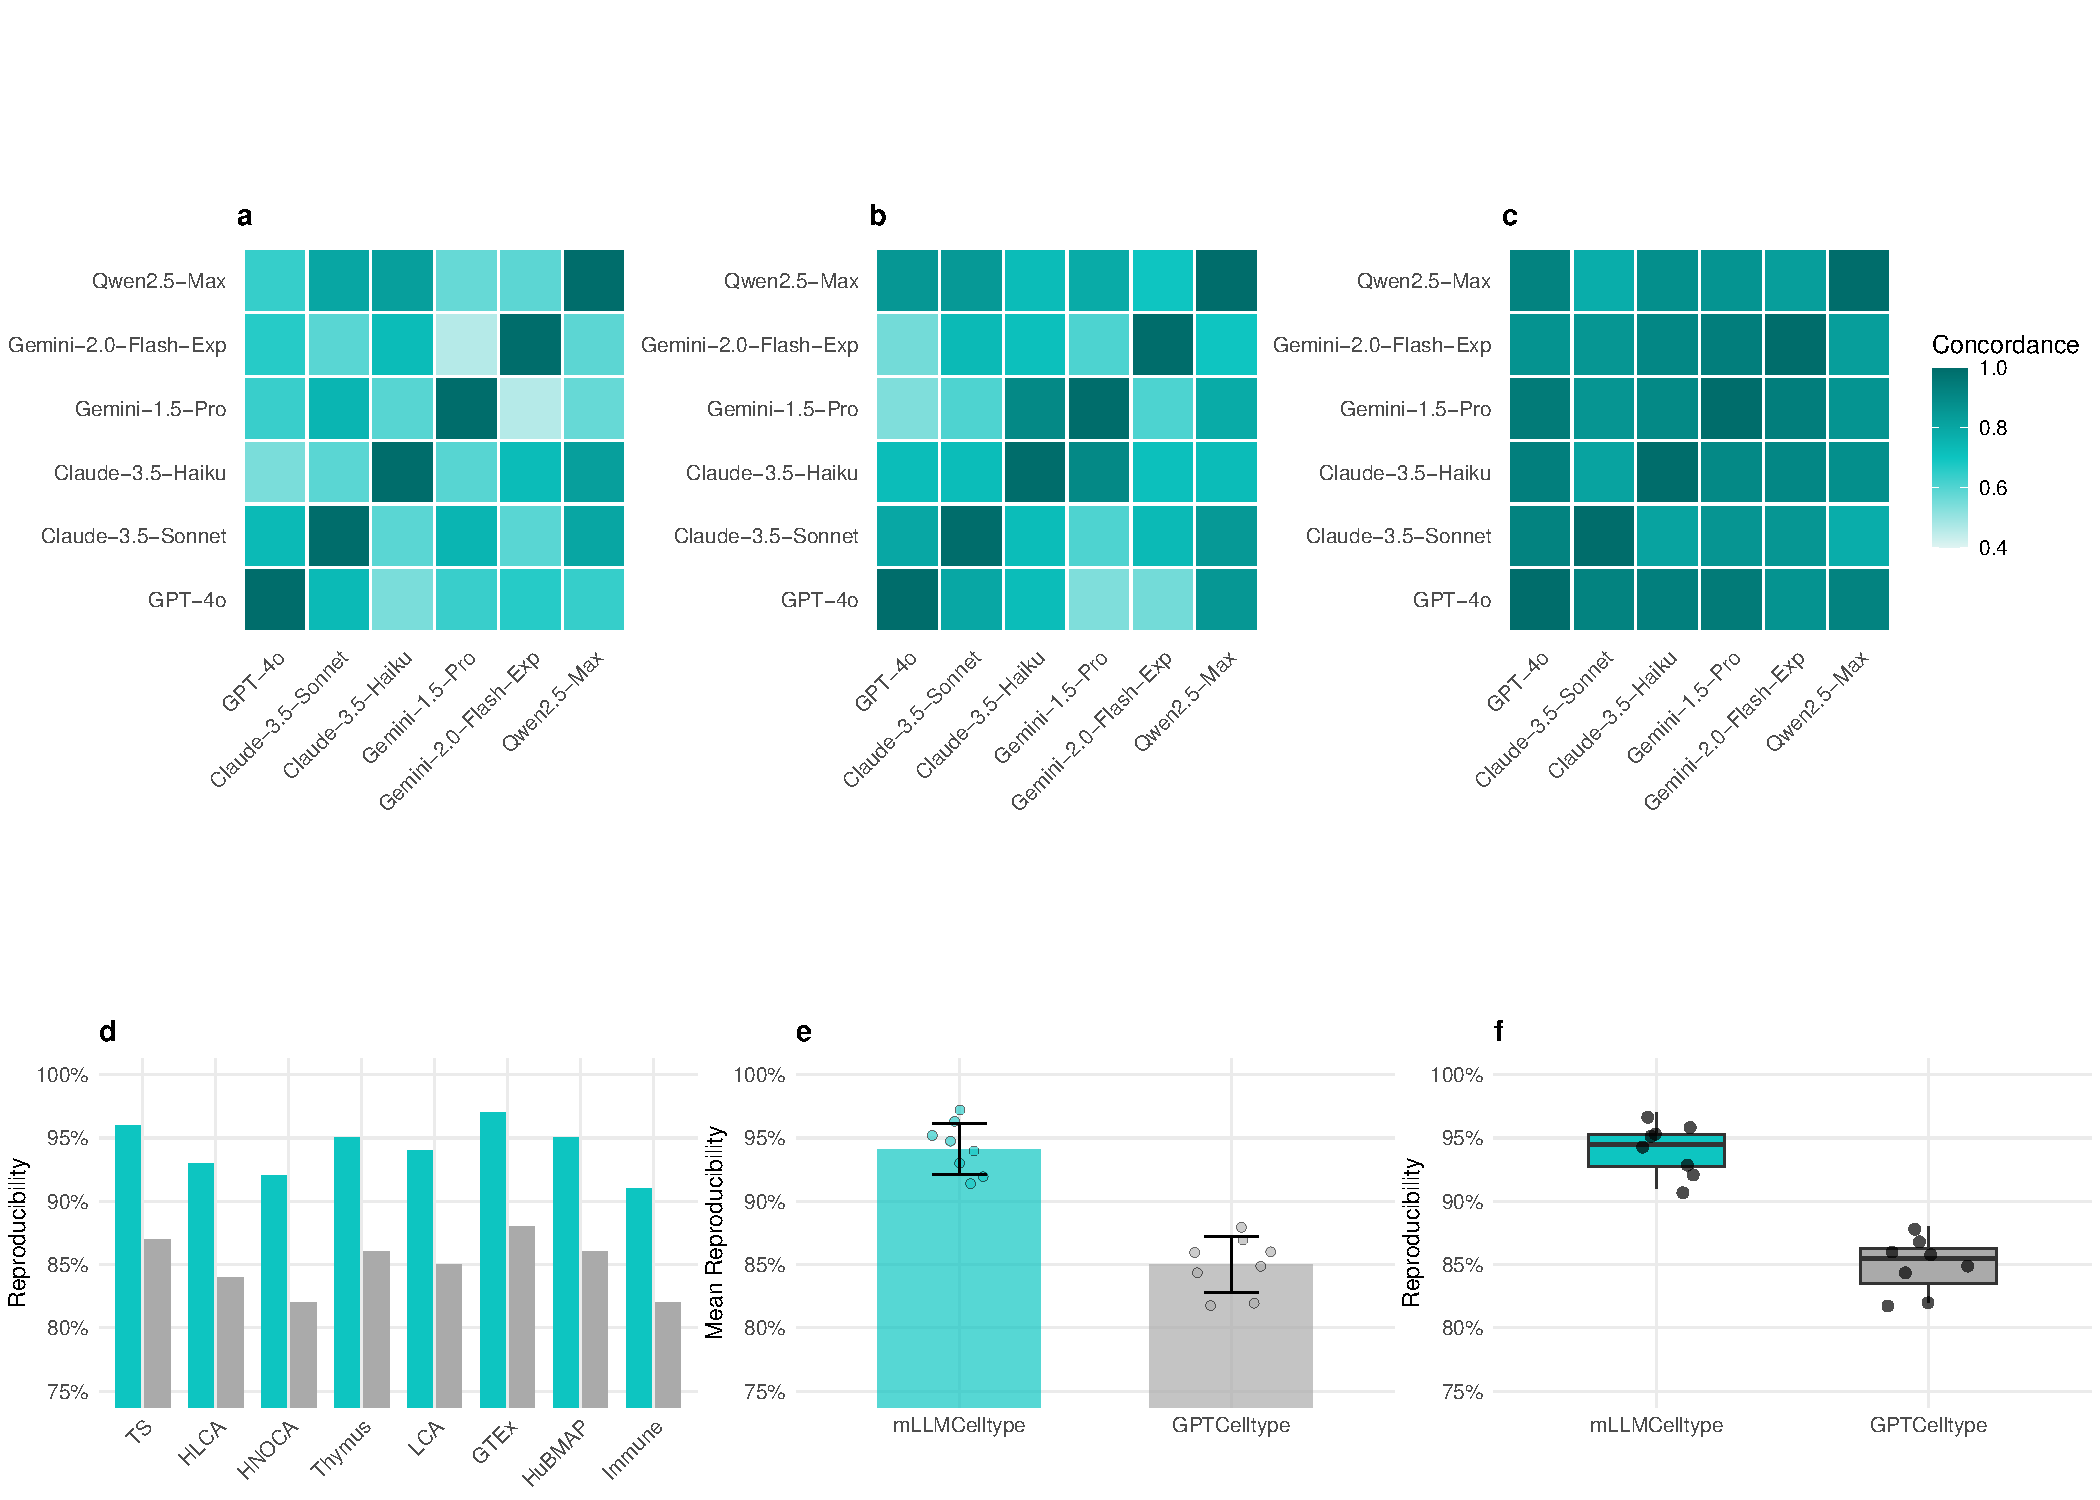
\includegraphics[width=\textwidth]{figures/supplementary_figure1.pdf}

\textbf{a--c}, Heatmaps showing pairwise concordance proportion between different LLMs across deliberation rounds. \textbf{a}, Initial concordance based on round 1 predictions. \textbf{b}, Increased concordance following round 2 deliberation. \textbf{c}, High concordance achieved in round 3, signifying convergence towards consensus. Results shown were generated using the TS dataset.

\textbf{d--f}, Reproducibility comparison between mLLMCelltype and GPTCelltype across 5 independent runs. \textbf{d}, Per-dataset reproducibility (proportion of cells receiving identical annotations across runs). \textbf{e}, Mean reproducibility with standard deviation error bars. \textbf{f}, Distribution of reproducibility scores. mLLMCelltype achieves 94.2\% mean reproducibility compared to 85\% for GPTCelltype, demonstrating that multi-model consensus effectively mitigates LLM stochasticity.
\end{figure}

\clearpage

\begin{figure}[!htbp]
\centering
\caption*{\textbf{Supplementary Figure 2 | HNOCA dataset annotation results comparison.}}
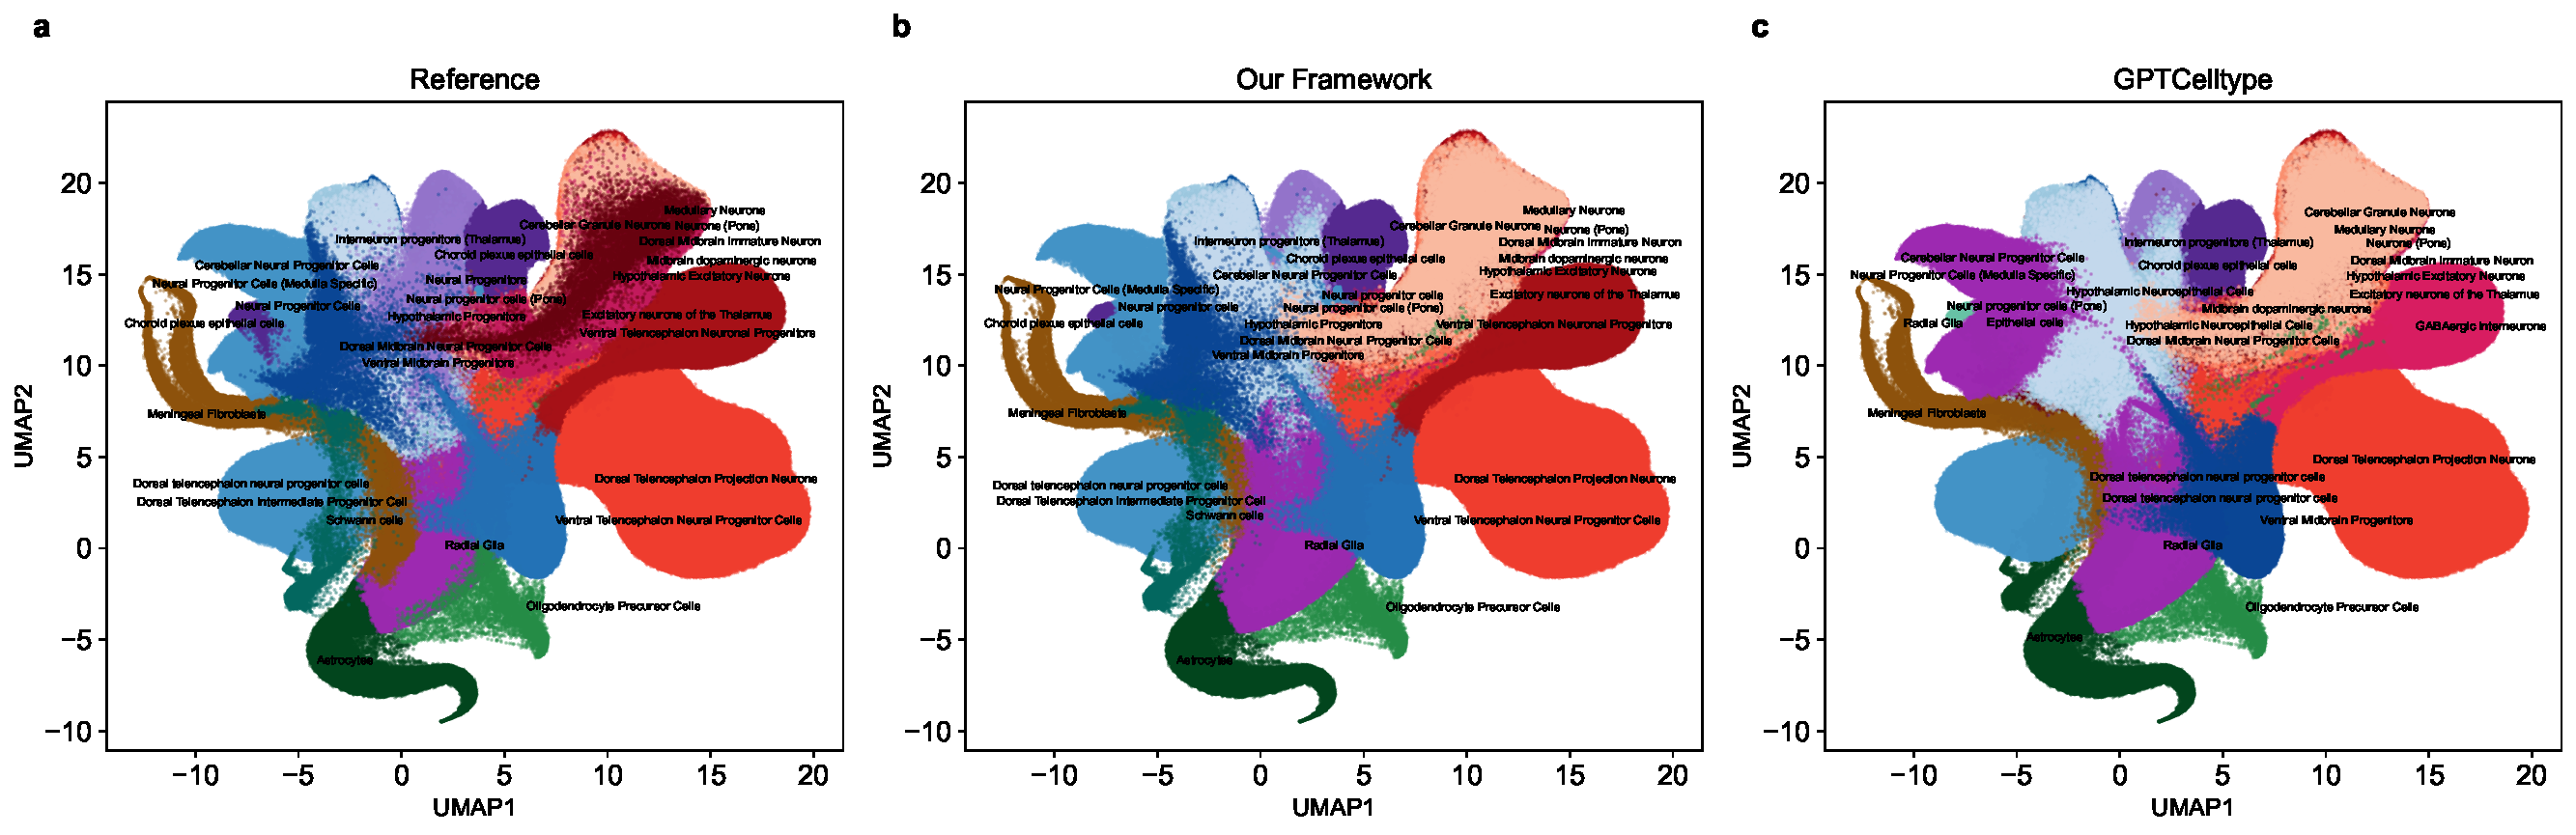
\includegraphics[width=\textwidth]{figures/supplementary_figure2.pdf}

\textbf{a}, UMAP visualization of HNOCA reference annotations showing major neural cell type populations and developmental states. The reference annotations were generated through a multi-step process using the snapseed tool, a marker-based hierarchical annotation method that combines cell type definitions, marker gene scoring, and reference mapping to human developmental brain atlases. The data was further refined through scPoli integration and label transfer from reference brain atlases using scVI and scANVI, particularly for non-telencephalic neurons and progenitor cells.

\textbf{b}, UMAP visualization of our framework's annotations demonstrating robust performance in identifying diverse neural cell types and developmental states, with high annotation accuracy when evaluated against reference annotations across this large-scale integrated atlas.

\textbf{c}, UMAP visualization of GPTCelltype annotations showing lower accuracy compared to our framework, particularly in distinguishing between closely related neural progenitor states and specialized neuronal subtypes.
\end{figure}

\clearpage

\begin{figure}[!htbp]
\centering
\caption*{\textbf{Supplementary Figure 3 | Annotation performance on the lifespan-wide human peripheral immune cell atlas.}}
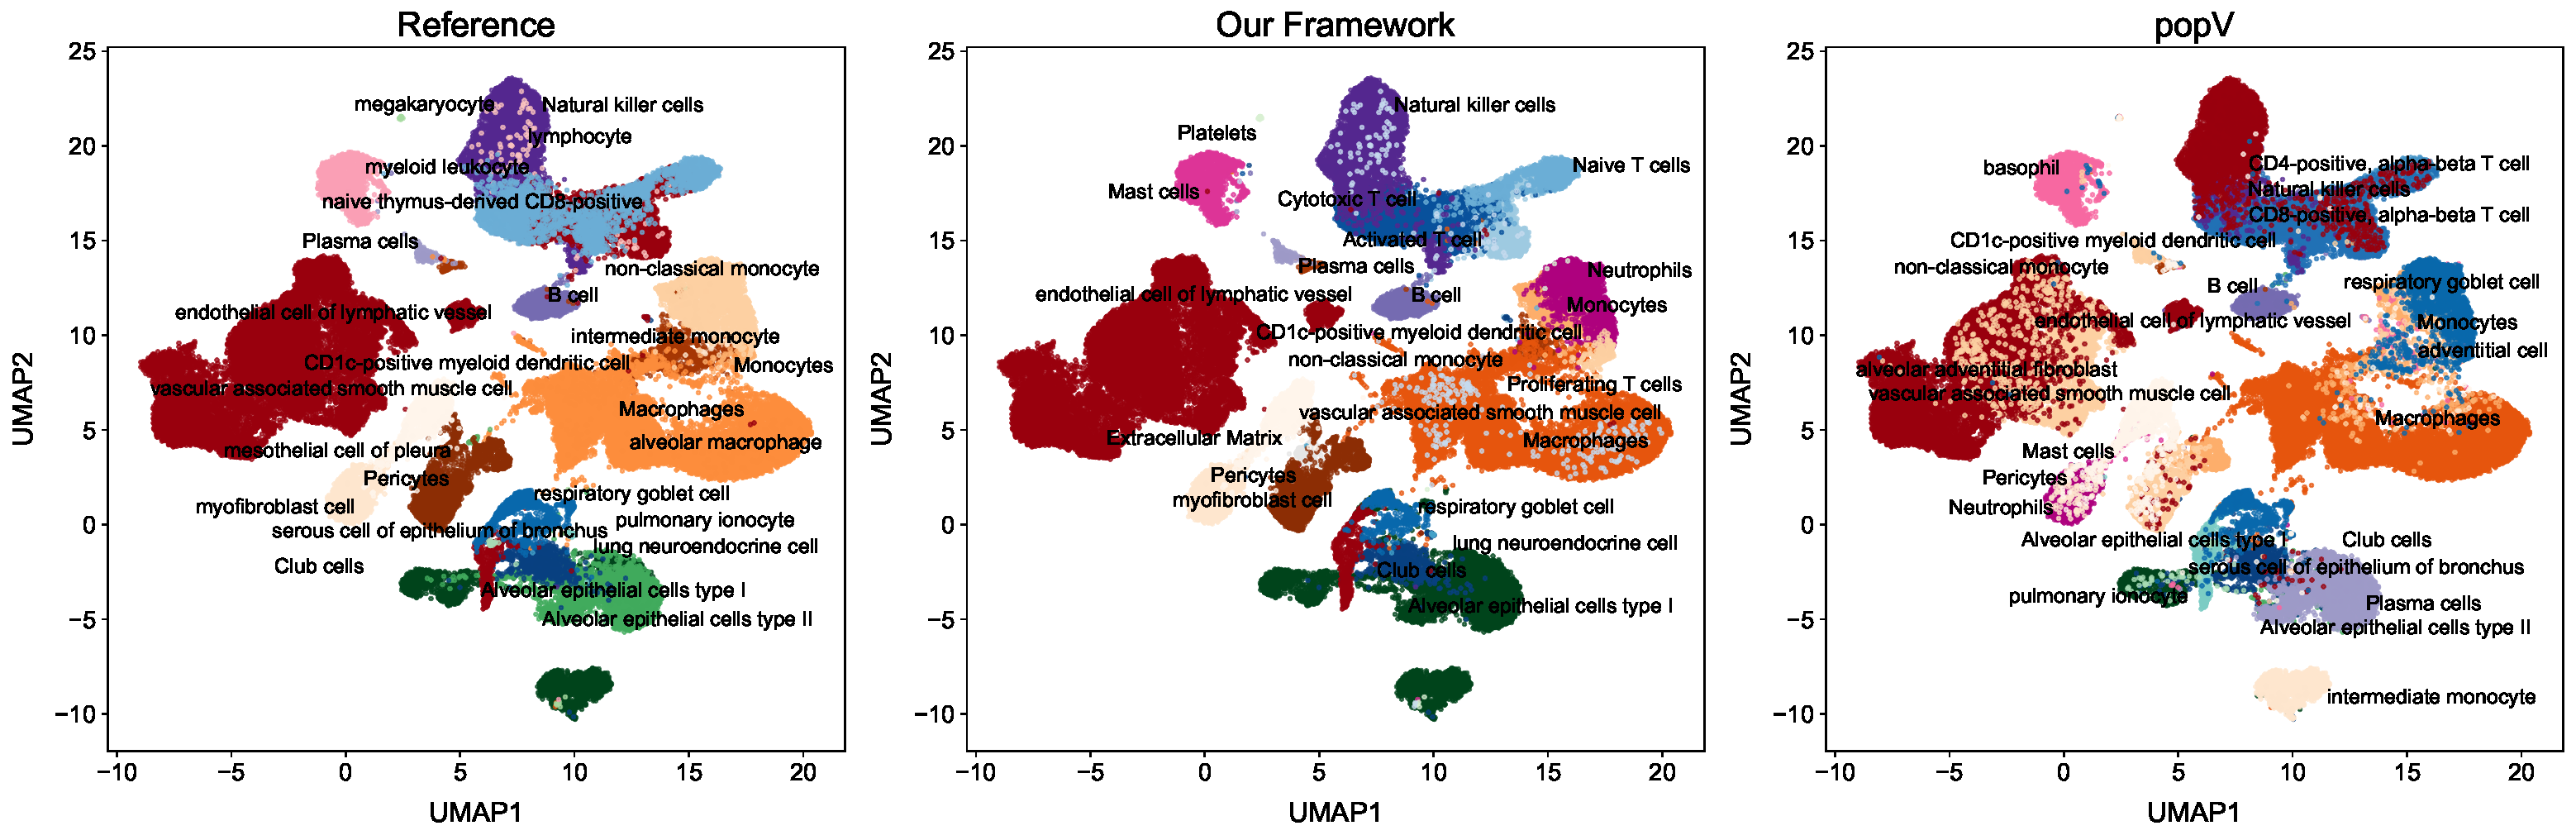
\includegraphics[width=\textwidth]{figures/supplementary_figure3.pdf}

\textbf{a}, UMAP visualization of reference annotations showing the distribution of immune cell types across the human lifespan. The reference annotations were generated through a comprehensive analysis of immune cells from 220 healthy donors spanning 13 age groups from birth to over 90 years, combining transcriptomic profiles with expert annotation.

\textbf{b}, UMAP visualization of our framework's annotations demonstrating high annotation accuracy (76.6\%) when evaluated against reference annotations, successfully capturing the complex developmental transitions and diverse immune cell populations.
\end{figure}

\clearpage

\begin{figure}[!htbp]
\centering
\caption*{\textbf{Supplementary Figure 4 | HLCA dataset annotation results comparison.}}
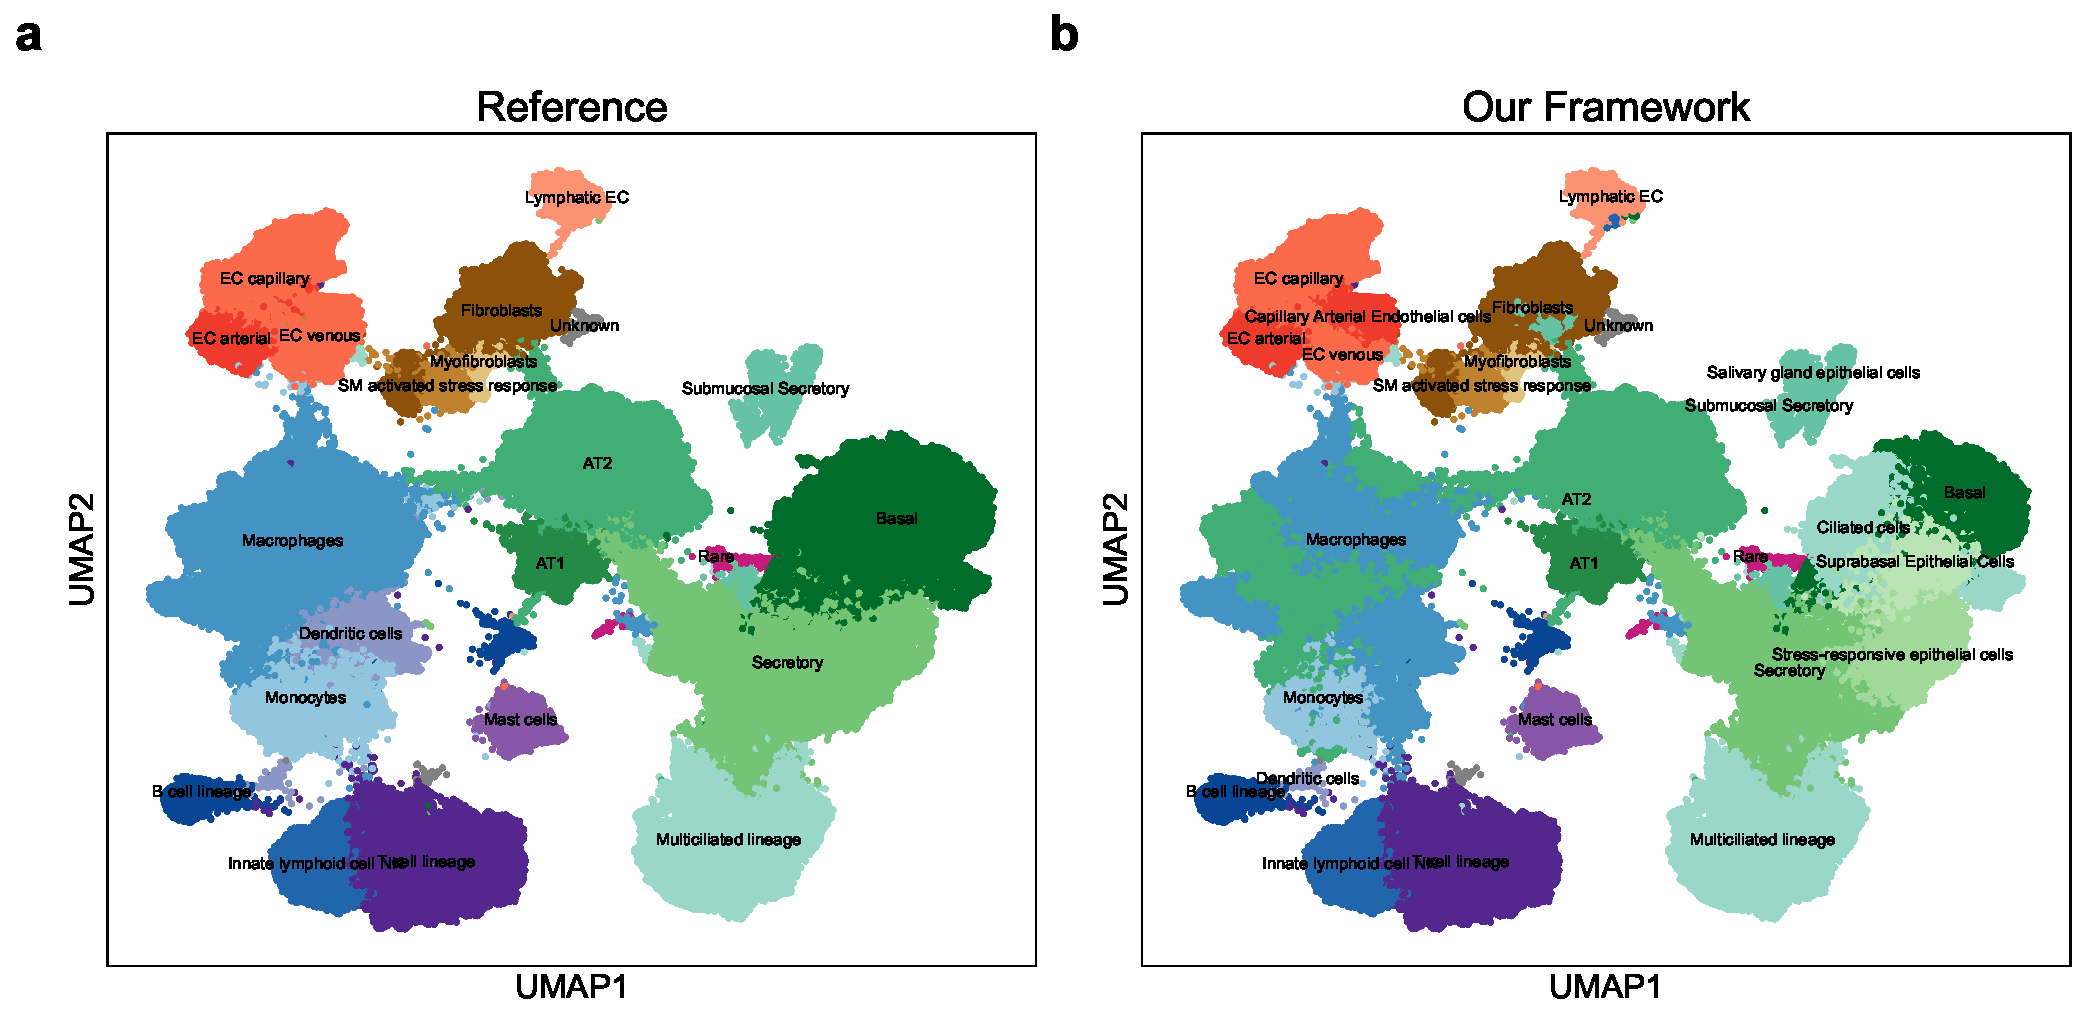
\includegraphics[width=\textwidth]{figures/supplementary_figure4.pdf}

\textbf{a}, UMAP visualization of HLCA reference annotations showing major cell type populations and their distribution. The HLCA reference annotations were generated through a hierarchical framework comprising 5 levels of granularity, from broad labels (Level 1: immune, epithelial, etc.) to fine-grained cell types (Level 5: e.g., naive CD4 T cells). The data integration and clustering were performed using scANVI, followed by Leiden clustering at different resolutions (Level 1: 0.01, Level 2: 0.2 with $k=30$, Levels 3-5: 0.2 with $k=15/10$). The final annotations were manually curated by six lung biology experts based on the clustering results, evidence from marker genes, and HLCA core clustering outcomes.

\textbf{b}, UMAP visualization of our framework's annotations demonstrating high annotation accuracy when evaluated against reference annotations. HLCA was analyzed using the hierarchical annotation strategy with sister cluster markers, as it met the criteria for this optional extension (explicit multi-level hierarchical structure, 5 levels of granularity, 58 fine-grained cell types at Level 4). HLCA was the only dataset meeting these criteria; all 49 benchmark datasets were analyzed using the core framework without hierarchical markers. Following the same hierarchical clustering approach as the reference, our framework performed cell type annotation level by level. At each level, the LLMs were provided with global marker genes and sister marker genes, along with the parent cluster's annotation from the previous level to guide the annotation process. The effectiveness of incorporating sister cluster markers is demonstrated in Supplementary Figure 7, which shows 4.8\% average accuracy improvement compared to using global markers alone.
\end{figure}

\clearpage

\begin{figure}[!htbp]
\centering
\caption*{\textbf{Supplementary Figure 5 | Performance on alternative single-cell sequencing platforms.}}
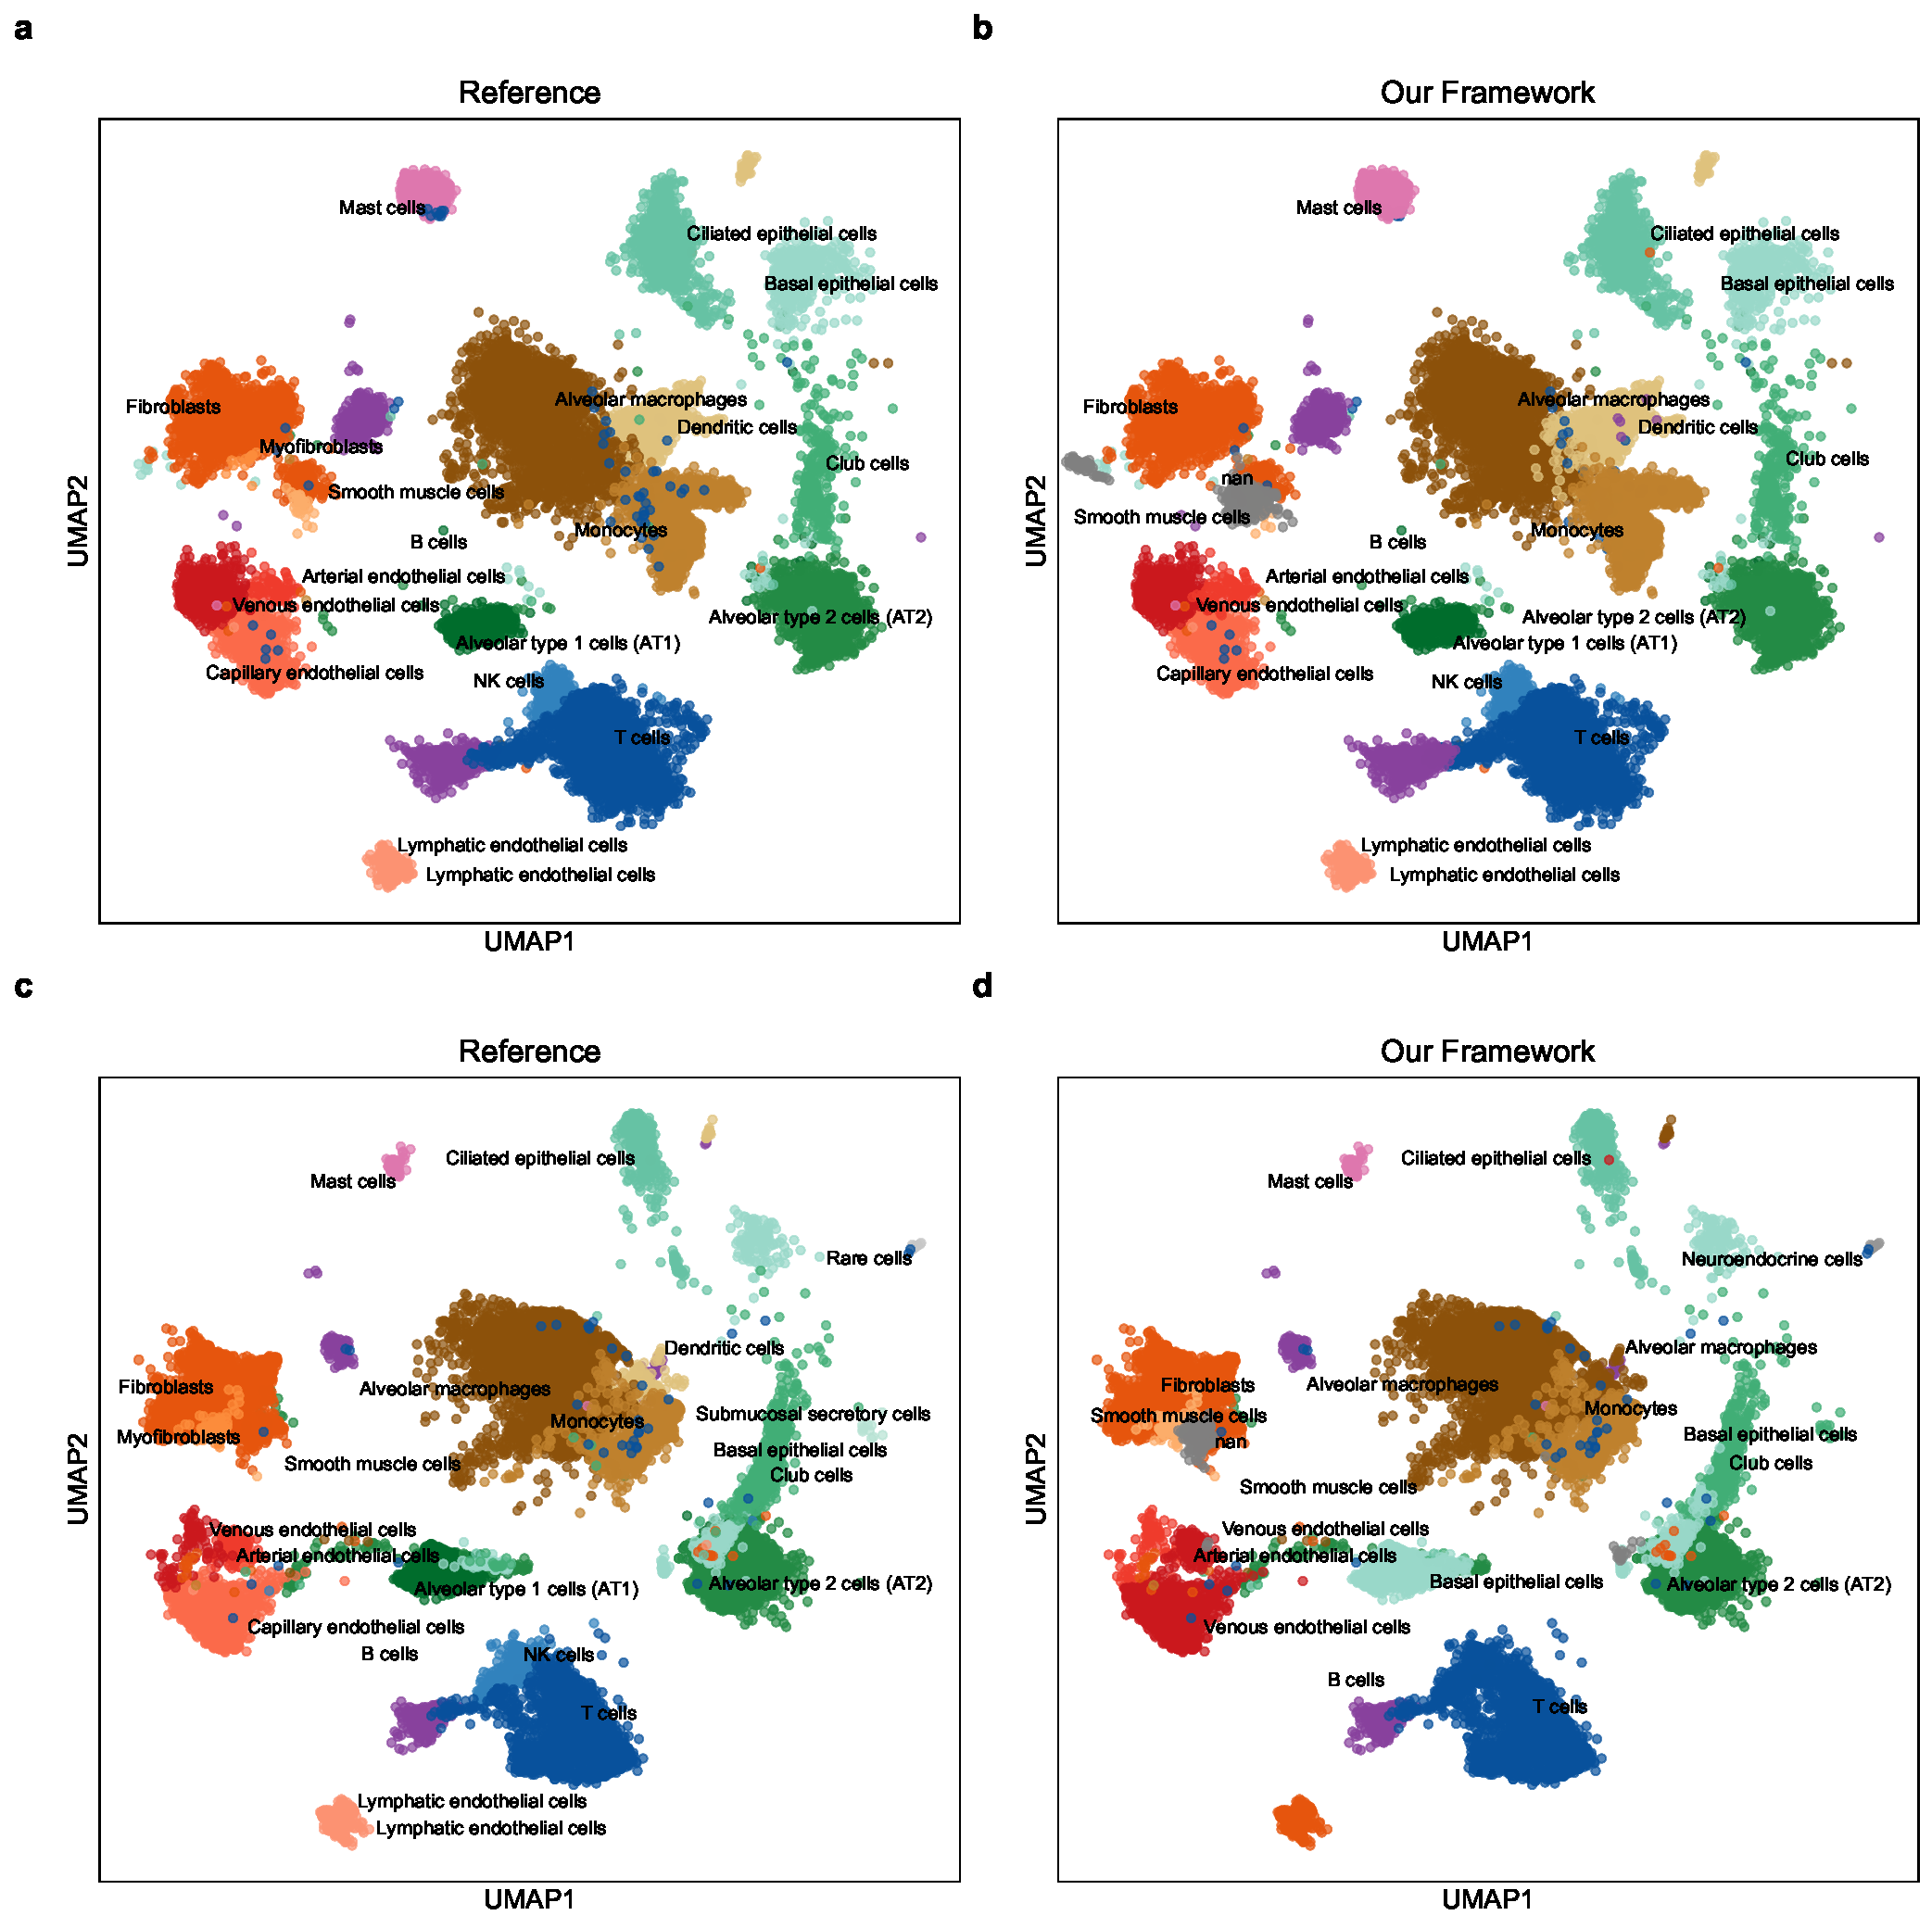
\includegraphics[width=\textwidth]{figures/supplementary_figure5.pdf}

\textbf{a}, UMAP visualization of reference annotations from Drop-seq data, demonstrating the distribution of cell populations in this alternative sequencing platform.

\textbf{b}, UMAP visualization of our framework's annotations on Drop-seq data showing 95\% annotation accuracy with reference annotations.

\textbf{c}, UMAP visualization of reference annotations from snRNA-seq data, showing cell type distributions in the snRNA-seq platform.

\textbf{d}, UMAP visualization of our framework's annotations on snRNA-seq data demonstrating robust performance across different nuclear transcriptome profiles, validating our framework's applicability to diverse scRNA-seq technologies.
\end{figure}

\clearpage

\begin{figure}[!htbp]
\centering
\caption*{\textbf{Supplementary Figure 6 | Optimization of marker gene selection for multi-LLM annotation framework.}}
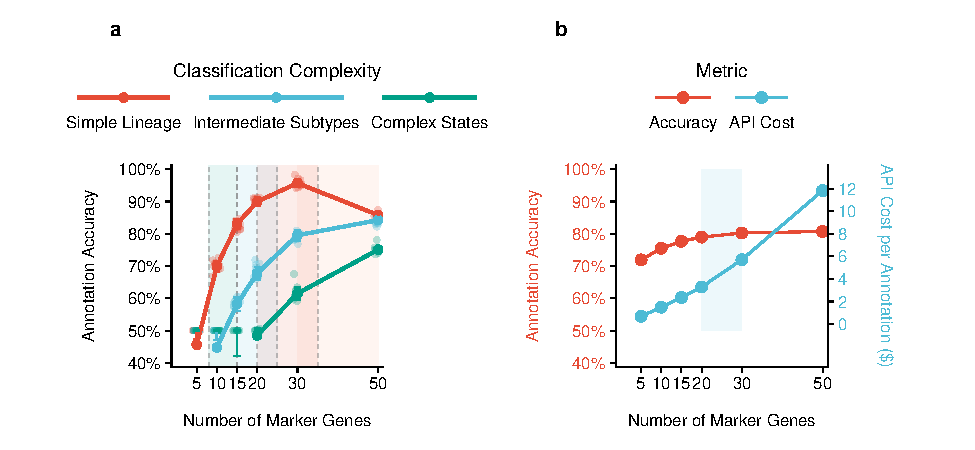
\includegraphics[width=\textwidth]{figures/supplementary_figure6.pdf}

\textbf{a}, Quantitative assessment of annotation accuracy as a function of the number of marker genes across different classification complexities using the Tabula Sapiens (TS) dataset. Three distinct complexity levels are shown: simple lineage classification (red line, e.g., B/T cell distinction), intermediate subtypes (blue line, e.g., T cell subtypes such as CD4+/CD8+), and complex states (green line, e.g., naive/memory/effector states). Performance curves demonstrate the optimal ranges: simple lineage classification (8--15 marker genes), intermediate complexity (15--25 marker genes), and complex developmental states (20--35 marker genes). Each data point represents the annotation accuracy, with error bars showing standard deviation. The shaded region beyond 30 marker genes indicates potential diminishing returns and increased complexity.

\textbf{b}, Annotation accuracy and cost at different numbers of marker genes. The primary axis (red) shows annotation accuracy, while the secondary axis (blue) tracks API cost per annotation. The blue-shaded region (20--30 marker genes) highlights the range that balances accuracy with cost.
\end{figure}

\clearpage

\begin{figure}[!htbp]
\centering
\caption*{\textbf{Supplementary Figure 7 | Impact of sister marker genes in hierarchical annotation strategy.}}
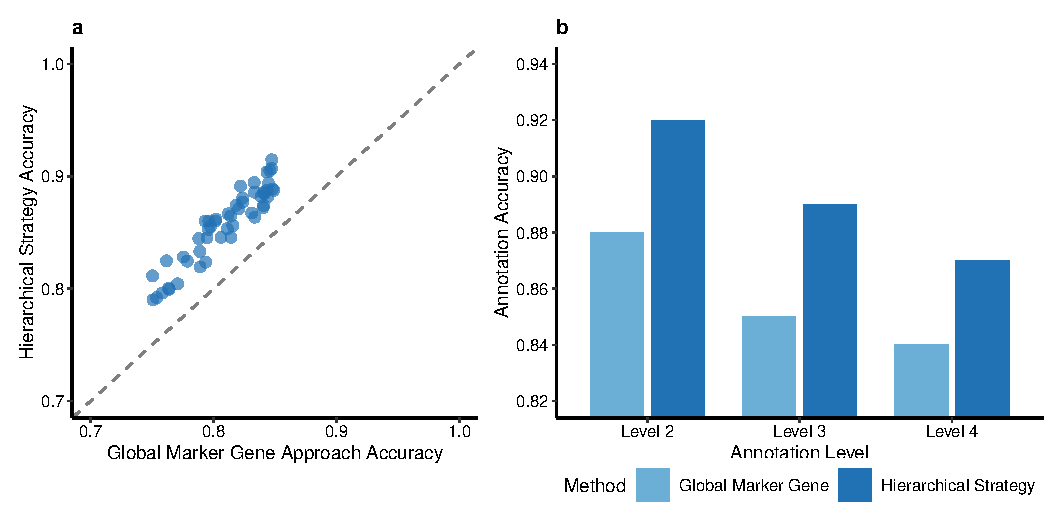
\includegraphics[width=\textwidth]{figures/supplementary_figure7.pdf}

\textbf{a}, Comparison of annotation accuracy at Level 4 between two hierarchical input strategies using the Human Lung Cell Atlas (HLCA) dataset. The strategies compared are: `Global Markers Only' (genes differentiating the cluster from all others at the current level, along with parent annotation) versus `Global + Sister Markers' (adding genes that differentiate the cluster specifically from its siblings within the same parent). The scatter plot shows consistent improvement across 50 repeated experiments when sister markers are included, with accuracy gains ranging from 3 to 7 percentage points and averaging 4.8\%.

\textbf{b}, Quantitative analysis showing the improvement in annotation accuracy across annotation levels (Level 2, Level 3, and Level 4) when sister marker genes are included. For instance, at Level 4, accuracy increased by 3 percentage points (from 84\% to 87\%) in this representative analysis when sister marker genes were included, contributing to the overall average improvement shown in panel a. This enhancement is particularly significant for resolving closely related subtypes which may share many global markers but exhibit key differences relative to their immediate siblings.
\end{figure}

\clearpage

\begin{figure}[!htbp]
\centering
\caption*{\textbf{Supplementary Figure 8 | Comparison with popV and scANVI across benchmark datasets.}}
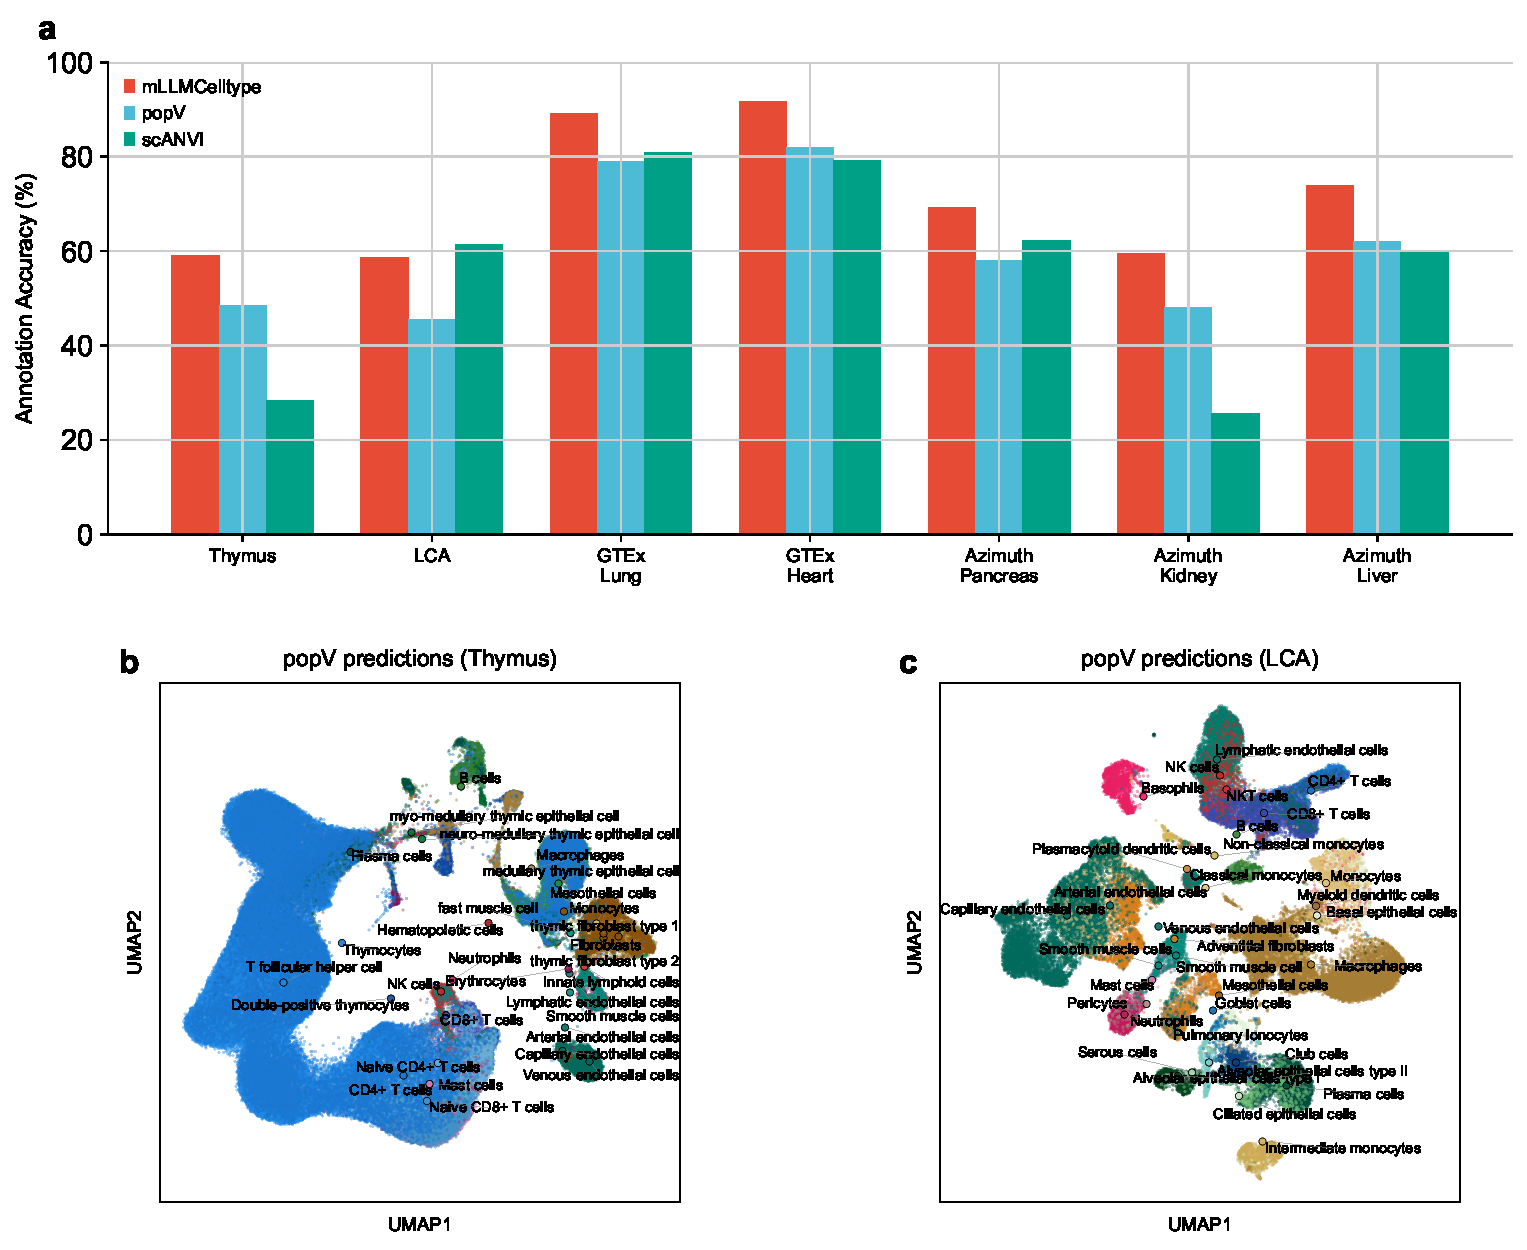
\includegraphics[width=\textwidth]{figures/supplementary_figure8.pdf}

\textbf{a}, Quantitative comparison of annotation accuracy between mLLMCelltype, popV, and scANVI across 7 representative datasets. Datasets span independent studies (Thymus, LCA), GTEx (Lung, Heart), and Azimuth references (Pancreas, Kidney, Liver). popV predictions used organ-specific Tabula Sapiens pretrained models. scANVI was trained on the corresponding Tabula Sapiens tissue reference for each dataset using scVI pretraining (100 epochs) followed by scANVI semi-supervised fine-tuning (20 epochs). mLLMCelltype outperforms scANVI on 5 of 7 datasets (mean 71.6\% vs.\ 56.7\%), with scANVI performing best on datasets where the Tabula Sapiens reference closely matches the query tissue (GTEx Lung: 80.8\%, GTEx Heart: 79.1\%).

\textbf{b}, UMAP visualization of popV annotations on the developmental human thymus dataset, using Tabula Sapiens Thymus as reference.

\textbf{c}, UMAP visualization of popV annotations on the Lung Cell Atlas (LCA) dataset, using Tabula Sapiens Lung as reference.
\end{figure}

\clearpage

\begin{figure}[!htbp]
\centering
\caption*{\textbf{Supplementary Figure 9 | Per-dataset comparison of annotation accuracy across all baseline methods.}}
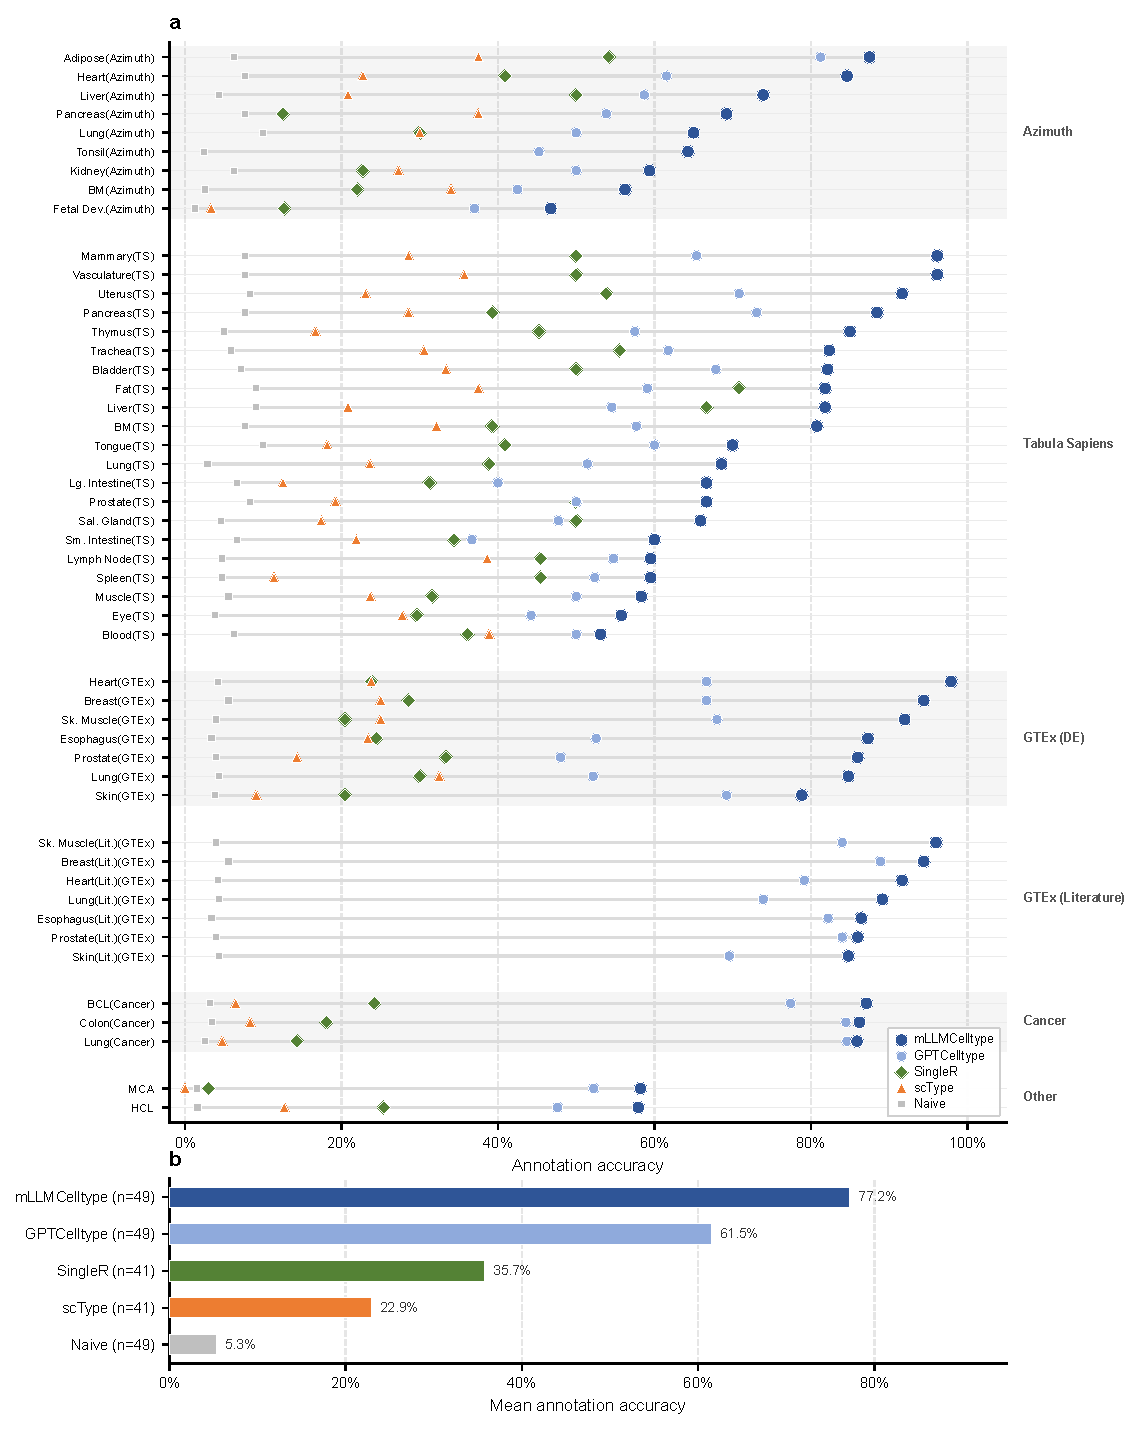
\includegraphics[width=\textwidth]{figures/supplementary_figure9.pdf}

\textbf{a}, Per-dataset annotation accuracy for five methods: mLLMCelltype, GPTCelltype, SingleR, scType, and a naive baseline (most-frequent cell type). Datasets are grouped by source category (Azimuth, Tabula Sapiens, GTEx, Cancer, Other). SingleR and scType bars are shown for the 41 benchmark datasets where expression matrices were available for reference-based evaluation (21 Tabula Sapiens tissues, 8 Azimuth reference datasets, 7 GTEx snRNA-seq tissues, MCA, 3 cancer datasets, and HCL), evaluated using HumanPrimaryCellAtlasData or MouseRNAseqData (SingleR) and ScTypeDB (scType) with Cell Ontology-aware accuracy scoring.

\textbf{b}, Summary of mean annotation accuracy across methods. Sample sizes are indicated in parentheses: SingleR and scType were evaluated on 41 of 49 datasets due to their dependence on reference atlases and marker databases, respectively. mLLMCelltype achieves the highest mean accuracy (77.2\%) across all 49 datasets, substantially outperforming all baselines.
\end{figure}

\end{document}